\documentclass[idioma,boletin]{uah}

\tema{5}
\titulo{Transmisión digital en banda base}{Baseband digital transmission}
%
\begin{document}

\titulacion{Grados TIC}
\asignatura{Teoría de la Comunicación}{Communication Theory}
\departamento{Teoría de la Señal y Comunicaciones}
\curso{2020/2021} % Do not show year

\maketitle


\Problema {

Un ordenador genera palabras binarias de $16$ bits a la velocidad de $20000$ palabras por segundo. 

\begin{enumerate}
	\item Calcule el ancho de banda necesario para transmitir la salida como una señal PAM binaria.
	\item Calcule $M$ para que la salida se pueda transmitir como señal $M$-aria en un canal de $B=60 kHz$.
\end{enumerate}

}
{

\begin{enumerate}
	\item $B_T \geq 160kHz$
	\item $M=8$
\end{enumerate}
}
{

A computer generates $16$-bits binary words, at $20000$ words per second. 

\begin{enumerate}
	\item Calculate the bandwidth necessary for transmitting the output as a PAM binary signal.
	\item Calculate $M$ so the output can be transmitted as an $M$-ary signal in a channel with $B=60 kHz$.
\end{enumerate}

}
{

\begin{enumerate}
	\item $B_T \geq 160kHz$
	\item $M=8$
\end{enumerate}
}


\Problema{

Considere una secuencia binaria $b_n$ a partir de la cual formamos los símbolos $a_n = b_n + b_{n-1}$. Los $b_n$ son variables aleatorias binarias incorreladas, que toman los valores $+1$ y $-1$ y tienen media cero y varianza unidad. 

Calcule la densidad espectral de potencia de la señal transmitida.
}
{

\begin{enumerate}
	\item $S_x(\omega) = \frac{4}{T} |H(\omega)|^2 cos^2 \left ( \omega \frac{T}{2} \right ) $
\end{enumerate}
}
{

Consider a binary sequence a $b_n$ from which we form the symbols $a_n = b_n + b_{n-1}$. Coefficients $b_n$ stand for uncorrelated random variables, which take values $+1$ and $-1$, with zero mean and variance 1. 

Calculate the power spectral density of the transmitted signal.

}
{

\begin{enumerate}
	\item $S_x(\omega) = \frac{4}{T} |H(\omega)|^2 cos^2 \left ( \omega \frac{T}{2} \right ) $
\end{enumerate}
}




\Problema {

Calcule la $\left ( \frac{S}{N} \right )_R$ para que un sistema binario unipolar con ruido blanco gaussiano aditivo tenga $P_e= 0.001$. 

¿Cuál será la probabilidad de error de un sistema polar con la misma $\left ( \frac{S}{N} \right )_R$.
}
{
\begin{enumerate}
	\item $\rho = \frac{E_s}{N_0/2} = 19,22$ \\
		$P_e = Q(4,38) < 8.54 \cdot 10^{-6}$
\end{enumerate}
}
{

Calculate the $\left ( \frac{S}{N} \right )_R$ such that a binary unipolar system with white Gaussian noise has a $P_e= 0.001$. 

What is the error probability of a polar system with the same $\left ( \frac{S}{N} \right )_R$?

}
{
\begin{enumerate}
	\item $\rho = \frac{E_s}{N_0/2} = 19,22$ \\
		$P_e = Q(4,38) < 8.54 \cdot 10^{-6}$
\end{enumerate}
}


\newpage


\Problema {

Considere la señal $h_{TC}(t)$ de la figura:

{\begin{figure*}[h!]\centering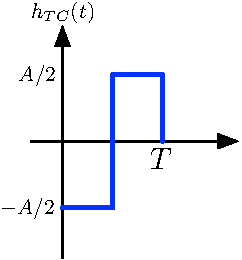
\includegraphics[width=4cm]{./Figuras/Problema5_4}\end{figure*}}

\begin{enumerate}
	\item Determine la respuesta al impulso del filtro adaptado a esta señal y represéntela en función del tiempo.
	\item Dibuje la forma de onda de la respuesta al impulso global $h(t)$.
\end{enumerate}
}
{
\begin{enumerate}
	\item $h_R(t) = h_{TC}(T-t)$
	\item \
	{\begin{figure*}[h!]\centering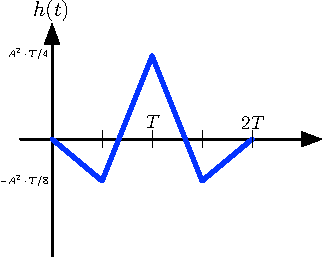
\includegraphics[width=4cm]{./Figuras/Problema5_4_sol}\end{figure*}}
\end{enumerate}
}
{

Consider the signal $h_{TC}(t)$ in the figure:

{\begin{figure*}[h!]\centering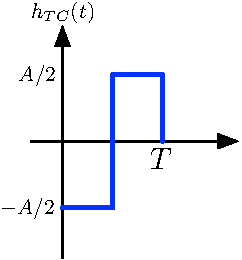
\includegraphics[width=4cm]{./Figuras/Problema5_4}\end{figure*}}

\begin{enumerate}
	\item Determine the impulse response of the matched filter to that signal, and draw it in function of the time.
	\item Draw the waveform of the global impulse response $h(t)$.

\end{enumerate}
}
{
\begin{enumerate}
	\item $h_R(t) = h_{TC}(T-t)$
	\item \
	{\begin{figure*}[h!]\centering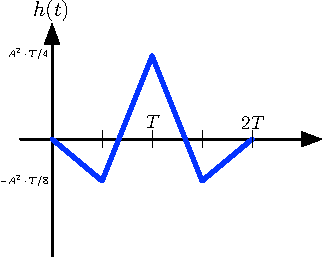
\includegraphics[width=4cm]{./Figuras/Problema5_4_sol}\end{figure*}}
\end{enumerate}
}

\newpage


\Problema {

Se recibe una señal PAM $r(t)=\sum_{n=-\infty}^{\infty} b_n h(t-nT)$.

 Dibuje dicha señal $r(t)$ y construya su diagrama de ojos, sin distorsión, para la siguiente secuencia de datos en formato unipolar: $1011100010$. 
 
 \begin{displaymath}
 	h(t) = cos^2 \left ( \frac{2\pi}{4T_b} t \right ) \prod \left ( \frac{t}{2T_b} \right )
 \end{displaymath}
}
{

{\begin{figure*}[h!]\centering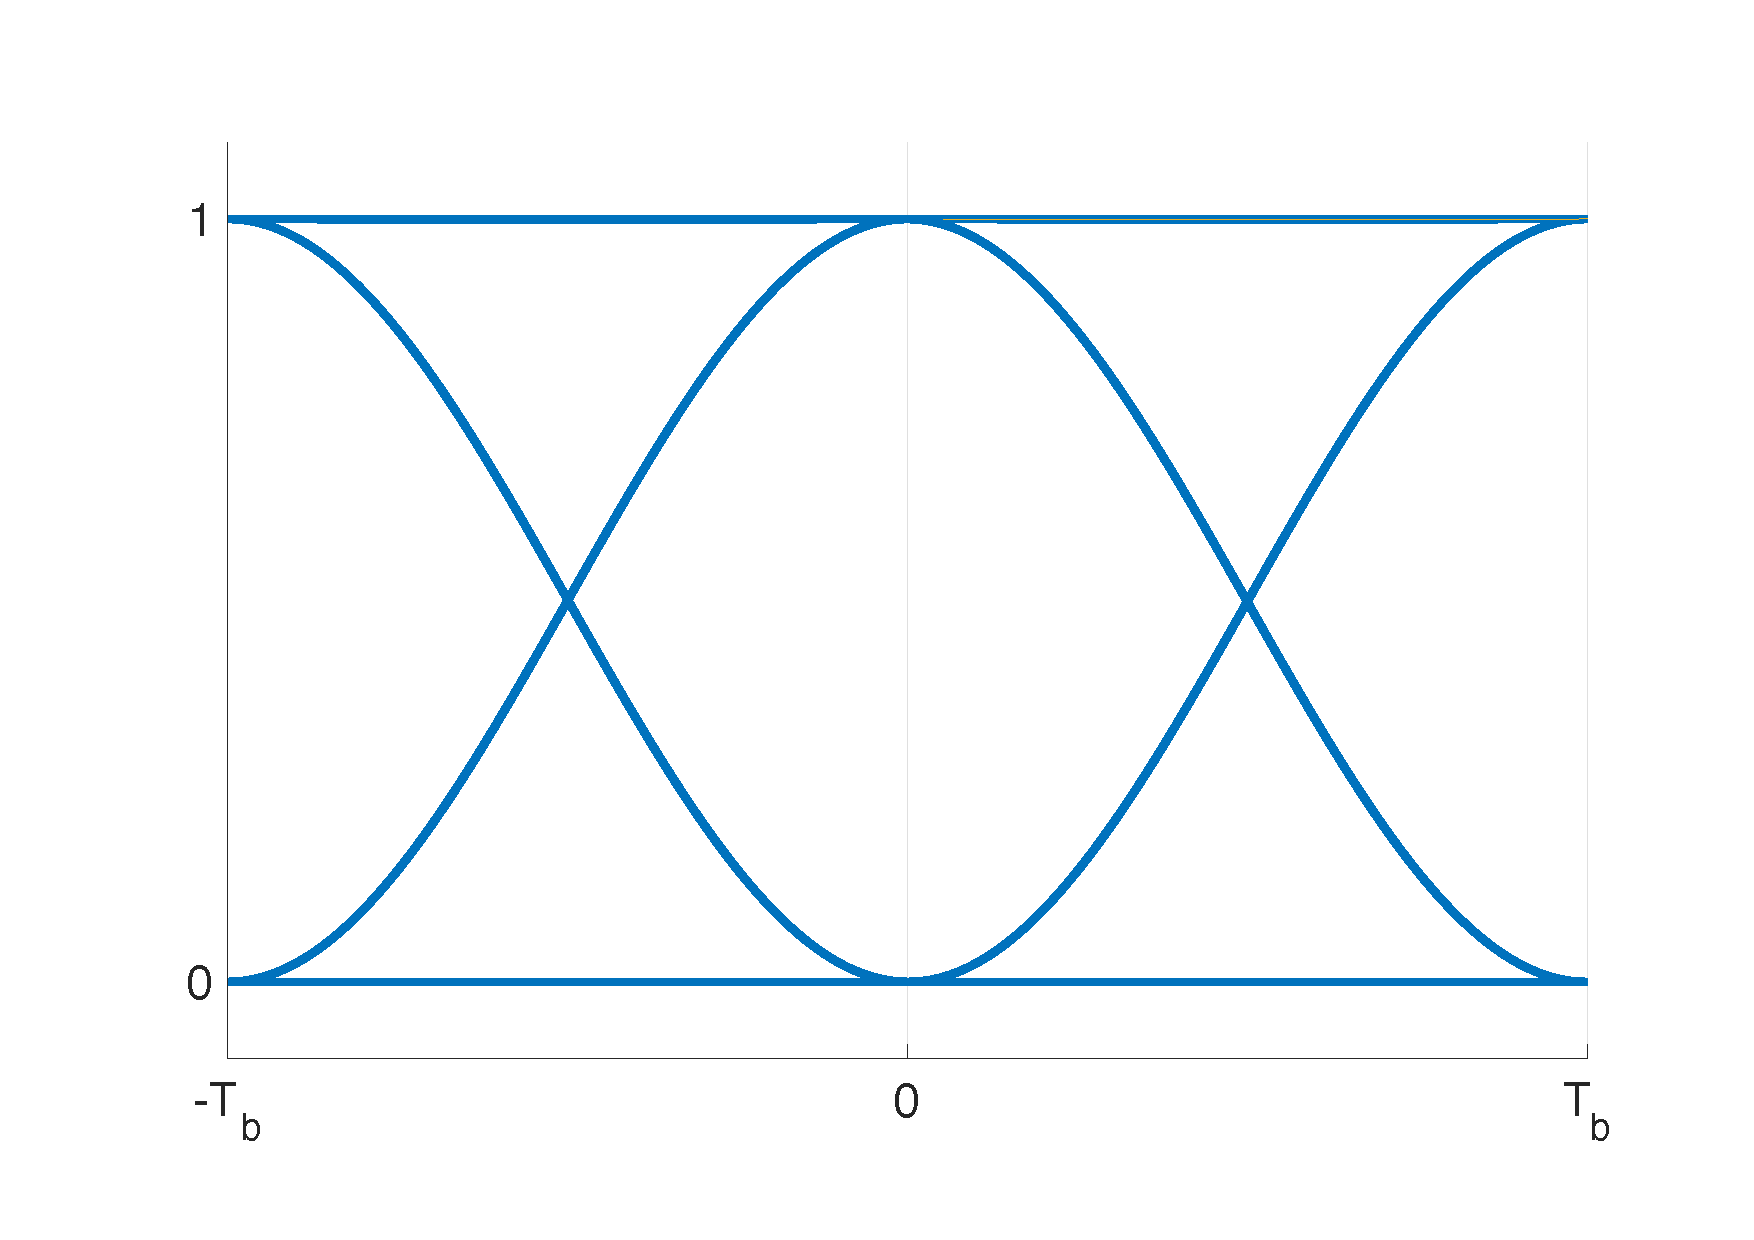
\includegraphics[width=8cm]{./Figuras/Problema5_5_sol}\end{figure*}}

}
{

The following PAM signal is received:  $r(t)=\sum_{n=-\infty}^{\infty} b_n h(t-nT)$.

 Draw and determine its eye pattern, without distortion, considering the following unipolar data sequence: $1011100010$. 
 
 \begin{displaymath}
 	h(t) = cos^2 \left ( \frac{2\pi}{4T_b} t \right ) \prod \left ( \frac{t}{2T_b} \right )
 \end{displaymath}
}
{

{\begin{figure*}[h!]\centering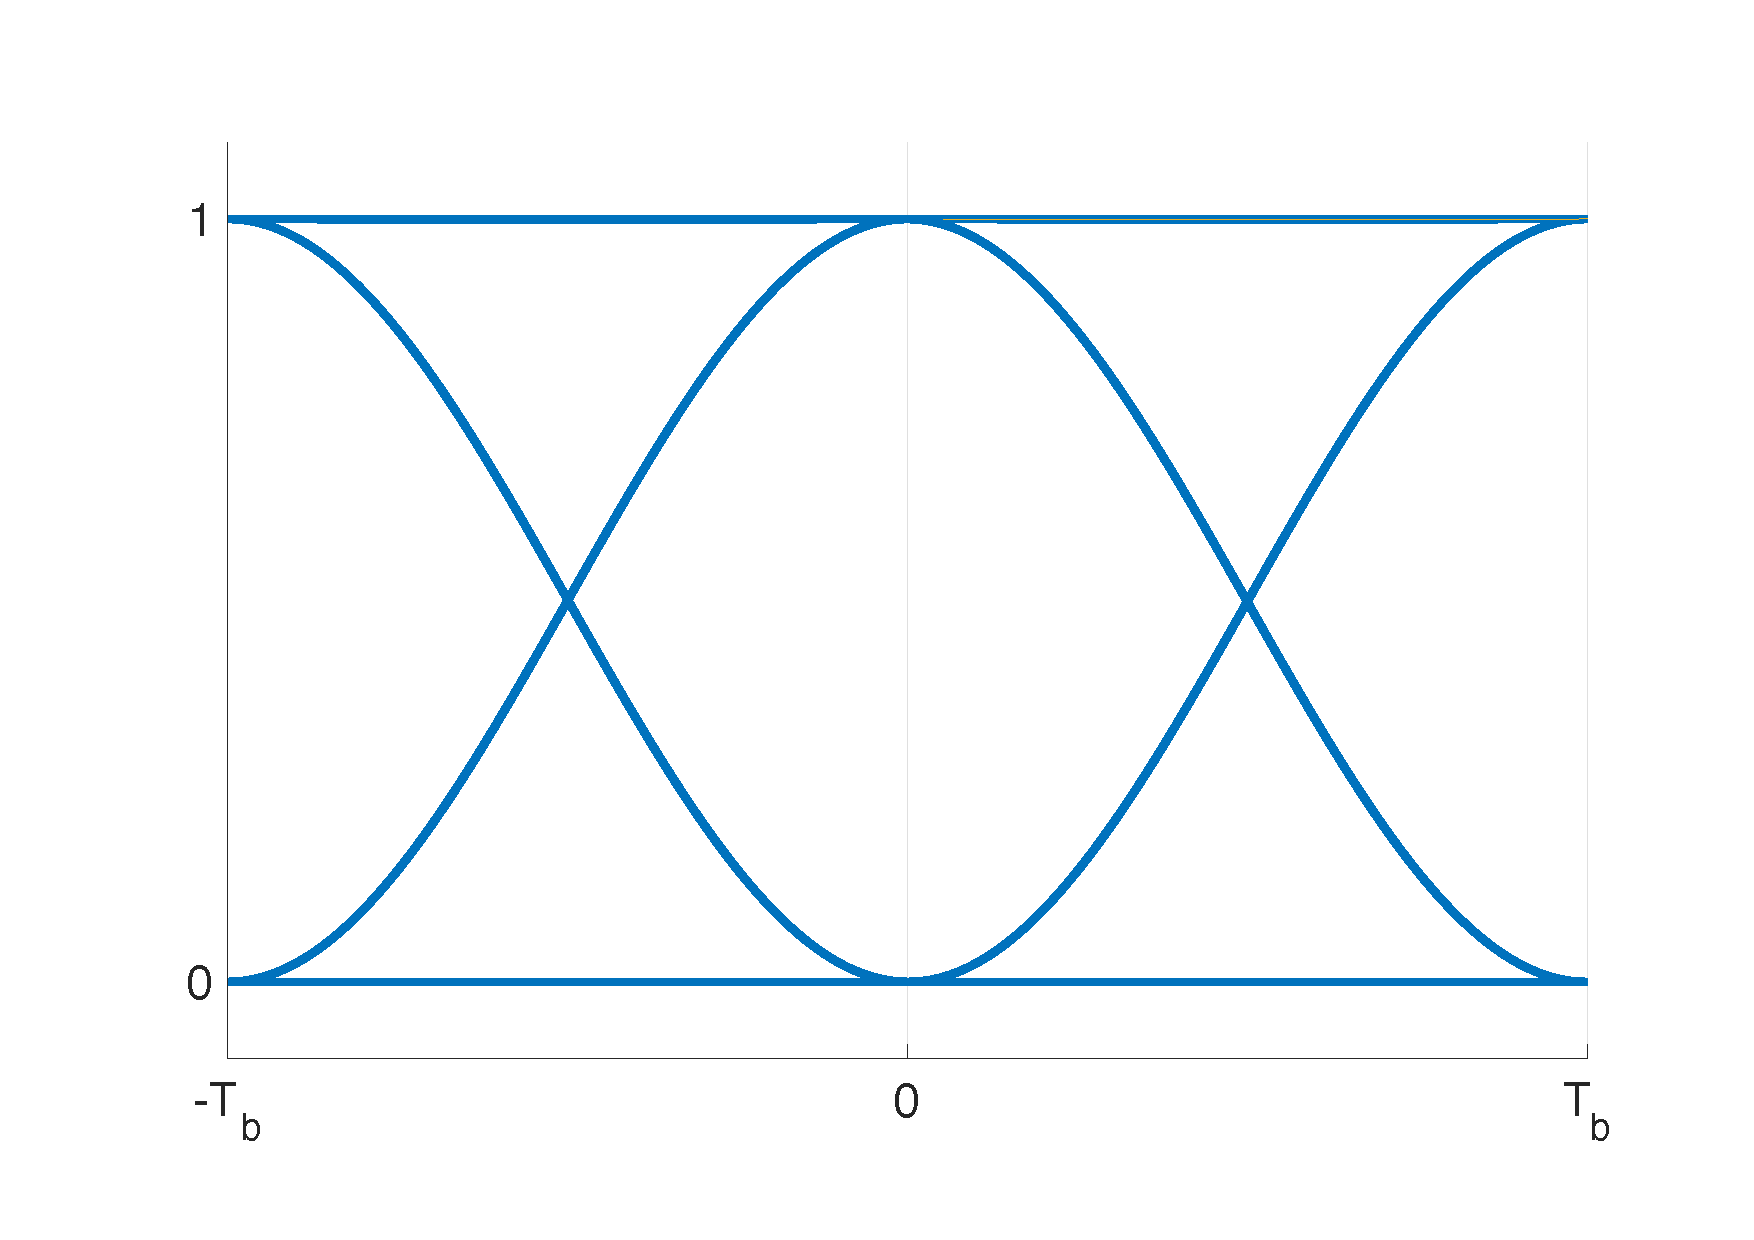
\includegraphics[width=8cm]{./Figuras/Problema5_5_sol}\end{figure*}}

}


\newpage

\Problema {

Un ordenador genera impulsos con una tasa de $R_b = 1 Mbps$, para su transmisión por un canal ruidoso con densidad espectral de potencia $N_0/2 = 2\cdot 10^{-20} W/Hz$. Se especifica que la tasa de error no debe superar el valor de $1$ bit por hora. Se pide:

\begin{enumerate}
	\item Determinar la potencia de ruido del canal y la probabilidad de error de bit en el sistema.
	\item Supóngase que en el transmisor se incluye ahora una característica de transferencia con espectro en coseno alzado, con un exceso de ancho de banda del $75\%$, y que el sistema sea PAM NRZ cuaternario. Calcular el nuevo ancho de banda necesario para la transmisión.
\end{enumerate}

}
{

\begin{enumerate}
	\item $P_N = 2 \cdot 10^{-14} W$, $P_b = 2.7 \cdot 10^{-10}$
	\item $B=437.5 kHz$
\end{enumerate}
}
{

A computer generates pulses with $R_b = 1 Mbps$, for their transmission through a noisy channel, with power spectral density $N_0/2 = 2\cdot 10^{-20} W/Hz$. The error rate cannot be over 1 bit per hour.

\begin{enumerate}
	\item Determine the noise power of the channel and the error probability of the system.
	\item Suppose that the transmitter includes now a transfer characteristic using a raised cosine spectrum, with an excess of bandwidth of $75\%$, and the systems is PAM NRZ quaternary. Calculate the new bandwidth necessary for the transmission.
\end{enumerate}

}
{

\begin{enumerate}
	\item $P_N = 2 \cdot 10^{-14} W$, $P_b = 2.7 \cdot 10^{-10}$
	\item $B=437.5 kHz$
\end{enumerate}
}



\Problema {

Un sistema de transmisión en banda base recibe la siguiente señal:

\begin{displaymath}
	r(t) = \sum_{n=-\infty}^{\infty} a_n \cdot h(t-nT)
\end{displaymath}

donde $T$ es el intervalo de símbolo, $a_n$ es una secuencia polar equiprobable incorrelada que puede tomar valores $-A$ o $+A$, y $h(t)$ corresponde a una forma de impulso en coseno alzado con roll-off factor  -exceso de ancho de banda- $\alpha$. 

Se pide:

\begin{enumerate}
	\item Calcular la densidad espectral de potencia de la señal recibida.
	\item Dar el ancho de banda de la misma.
\end{enumerate}
	
}
{

\begin{enumerate}
	\item $S_r(\omega) = \frac{1}{T} \cdot |H(\omega)|^2 \cdot A^2$ con $H(\omega)$ la respuesta en frecuencia del filtro en coseno alzado.
	\item $B = \pi \frac{1+\alpha}{T}$
\end{enumerate}
}
{

A base-band transmission system receives the following signal:

\begin{displaymath}
	r(t) = \sum_{n=-\infty}^{\infty} a_n \cdot h(t-nT)
\end{displaymath}

where $T$ stands for the symbol interval, an is a polar sequence equiprobable and uncorrelated, with values $-A$ or $+A$, and $h_T(t)$ corresponds to a pulse form in raised cosine, with roll-off factor $\alpha$.

\begin{enumerate}
	\item Calculate the power spectral density of the signal.
	\item Obtain the bandwidth.
\end{enumerate}
	
}
{

\begin{enumerate}
	\item $S_r(\omega) = \frac{1}{T} \cdot |H(\omega)|^2 \cdot A^2$ with $H(\omega)$ the frequency response of the raised cosine filter.
	\item $B = \pi \frac{1+\alpha}{T}$
\end{enumerate}
}


\newpage

\Problema{

Considere una secuencia binaria $b_n$ a partir de la cual formamos los símbolos $a_n= b_n - b_{n-1}$, los $b_n$ son variables aleatorias binarias equiprobables e incorreladas, que toman los valores $1$ y $0$. 

Calcule la densidad espectral de potencia de la señal transmitida para el caso en que el filtro transmisor tenga una respuesta al impulso:

\begin{displaymath}
	h_T(t) = \left \{ \begin{array}{ll}
		\frac{1}{\sqrt{T}} & 0 \leq t < T \\
		0 & c.c. \\
	\end{array} \right.
\end{displaymath}

}
{

$S_x(\omega) = \frac{4}{T^2 \omega^2} sen^4 \left ( \frac{\omega T}{2} \right )$
}
{

Consider a binary sequence $b_n$, from which we form the symbols $a_n= b_n - b_{n-1}$, $b_n$ are uncorrelated and equiprobable random variables, taking values $1$ and $0$. 

Calculate the power spectral density of the transmitted signal, in the case that the transmitter filter is:

\begin{displaymath}
	h_T(t) = \left \{ \begin{array}{ll}
		\frac{1}{\sqrt{T}} & 0 \leq t < T \\
		0 & c.c. \\
	\end{array} \right.
\end{displaymath}

}
{

$S_x(\omega) = \frac{4}{T^2 \omega^2} sen^4 \left ( \frac{\omega T}{2} \right )$
}

\newpage


\Problema {

Un sistema de comunicación digital tiene transmite la señal:

\begin{displaymath}
s(t) = \sum_{n=-\infty}^{\infty} b_n \cdot h_T(t-nT)
\end{displaymath}

donde $b_n$ representa una secuencia de variables aleatorias discretas, independientes e idénticamente distribuidas (iid) que toman valores $\pm 1$ con la misma probabilidad. La forma de onda del impulso transmitido es $h(t) = \frac{1}{\sqrt{T}} \cdot \prod \left ( \frac{t-T/2}{T} \right )$, la respuesta al impulso del canal es $h_c(t)=\delta (t)$ y el filtro receptor $h_R(t)$ está adaptado a $h_T(t)$. Se pide:

\begin{enumerate}
	\item Determinar la forma de onda de la respuesta al impulso global $h(t)$.
	\item Dibujar el diagrama de ojos de la señal de salida del filtro receptor antes de ser muestrada.
	\item Repetir el apartado a) para un canal con respuesta al impulso $h_c(t)=\delta (t) - 0.5 \cdot \delta (t-T)$.
	\item Calcular los valores de las muestras de la señal tomadas a la salida del filtro receptor, así como el valor de la interferencia entre símbolos (ISI) en cada una de ellas suponiendo que se ha transmitido la secuencia $1101$.
\end{enumerate}

\textsc{Nota:} $\prod(t) = \left \{ \begin{array}{ll} 1 & -0.5\leq t <0.5 \\ 0 & c.c. \\
 \end{array} \right.$
 \ \\

}
{

\begin{tabular}[h]{cc}
	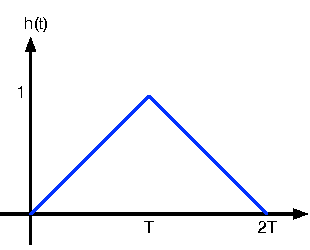
\includegraphics[height=2.5cm]{./Figuras/Problema5_9a} &
	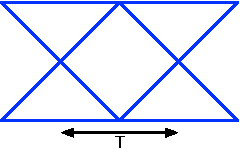
\includegraphics[height=1.75cm]{./Figuras/Problema5_9b} \\
	Apartado (a) & Apartado (b) \\
	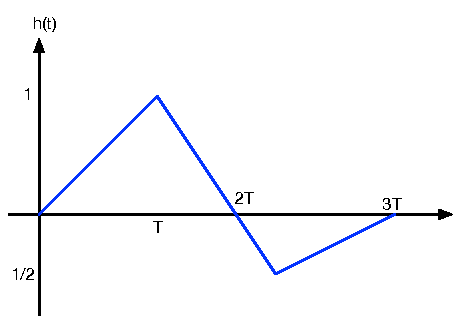
\includegraphics[height=2.5cm]{./Figuras/Problema5_9c} &
	\\
	Apartado (c) & \\
\end{tabular}

}
{

A communication system transmits the following signal:

\begin{displaymath}
s(t) = \sum_{n=-\infty}^{\infty} b_n \cdot h_T(t-nT)
\end{displaymath}

where $b_n$ represents a sequence of discrete random variables, independent and identically distributed, which take the values $\pm 1$ with the same probability. The transmitted pulse is $h(t) = \frac{1}{\sqrt{T}} \cdot \prod \left ( \frac{t-T/2}{T} \right )$, the channel impulse response is $h_c(t)=\delta (t)$ and the receiver filter $h_R(t)$ is matched to $h_T(t)$. Se pide:


	.
	
	
	

\begin{enumerate}
	\item Determine the wave form of the global impulse response $h(t)$.
	\item Draw the eye diagram of the receiver filter output, before sampling.
	\item Repeat a) for a channel with impulse response $h_c(t)=\delta (t) - 0.5 \cdot \delta (t-T)$.
	\item Calculate the values of the samples at the receiver filter output, and the value of the inter-symbol interference in each of them.
\end{enumerate}

\textsc{Note:} $\prod(t) = \left \{ \begin{array}{ll} 1 & -0.5\leq t <0.5 \\ 0 & c.c. \\
 \end{array} \right.$
 \ \\

}
{

\begin{tabular}[h]{cc}
	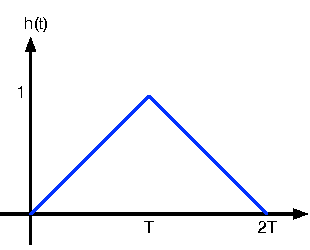
\includegraphics[height=2.5cm]{./Figuras/Problema5_9a} &
	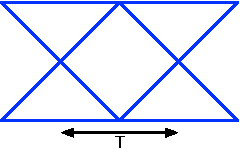
\includegraphics[height=1.75cm]{./Figuras/Problema5_9b} \\
	Apartado (a) & Apartado (b) \\
	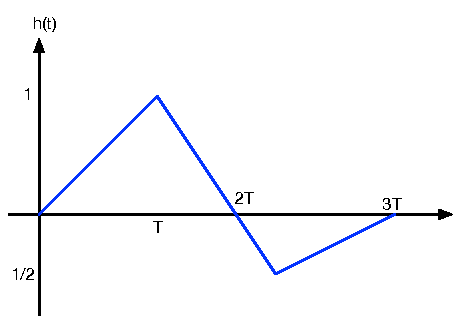
\includegraphics[height=2.5cm]{./Figuras/Problema5_9c} &
	\\
	Apartado (c) & \\
\end{tabular}

}



\end{document}



	
